\section{Robot} 

The robot is made using a Lego Mindstorm kit, with a NXT brick and a few different sensors, like light sensors, push sensors, etc. There was also a lot of Lego at disposal so there were free reins, construction wise. Sensor wise there were more limitations, i.e. only sensors from the given kit could be used.
\subsection{Behavior}

\subsection{Construction}
The skeleton of the robot was designed to be as low as possible, in order to get the light sensors as close to the ground as possible. A side effect of this is that it makes the robot more stable when turning. In front of the robot a gripper was placed, with room for two sensors in between the robot and the gripper. The final choice of design and sensor placement can be seen in figure \ref{fig:final_robot}. Other constructions was tried, but discarded for different reasons.

\begin{figure}[H]
\centering
 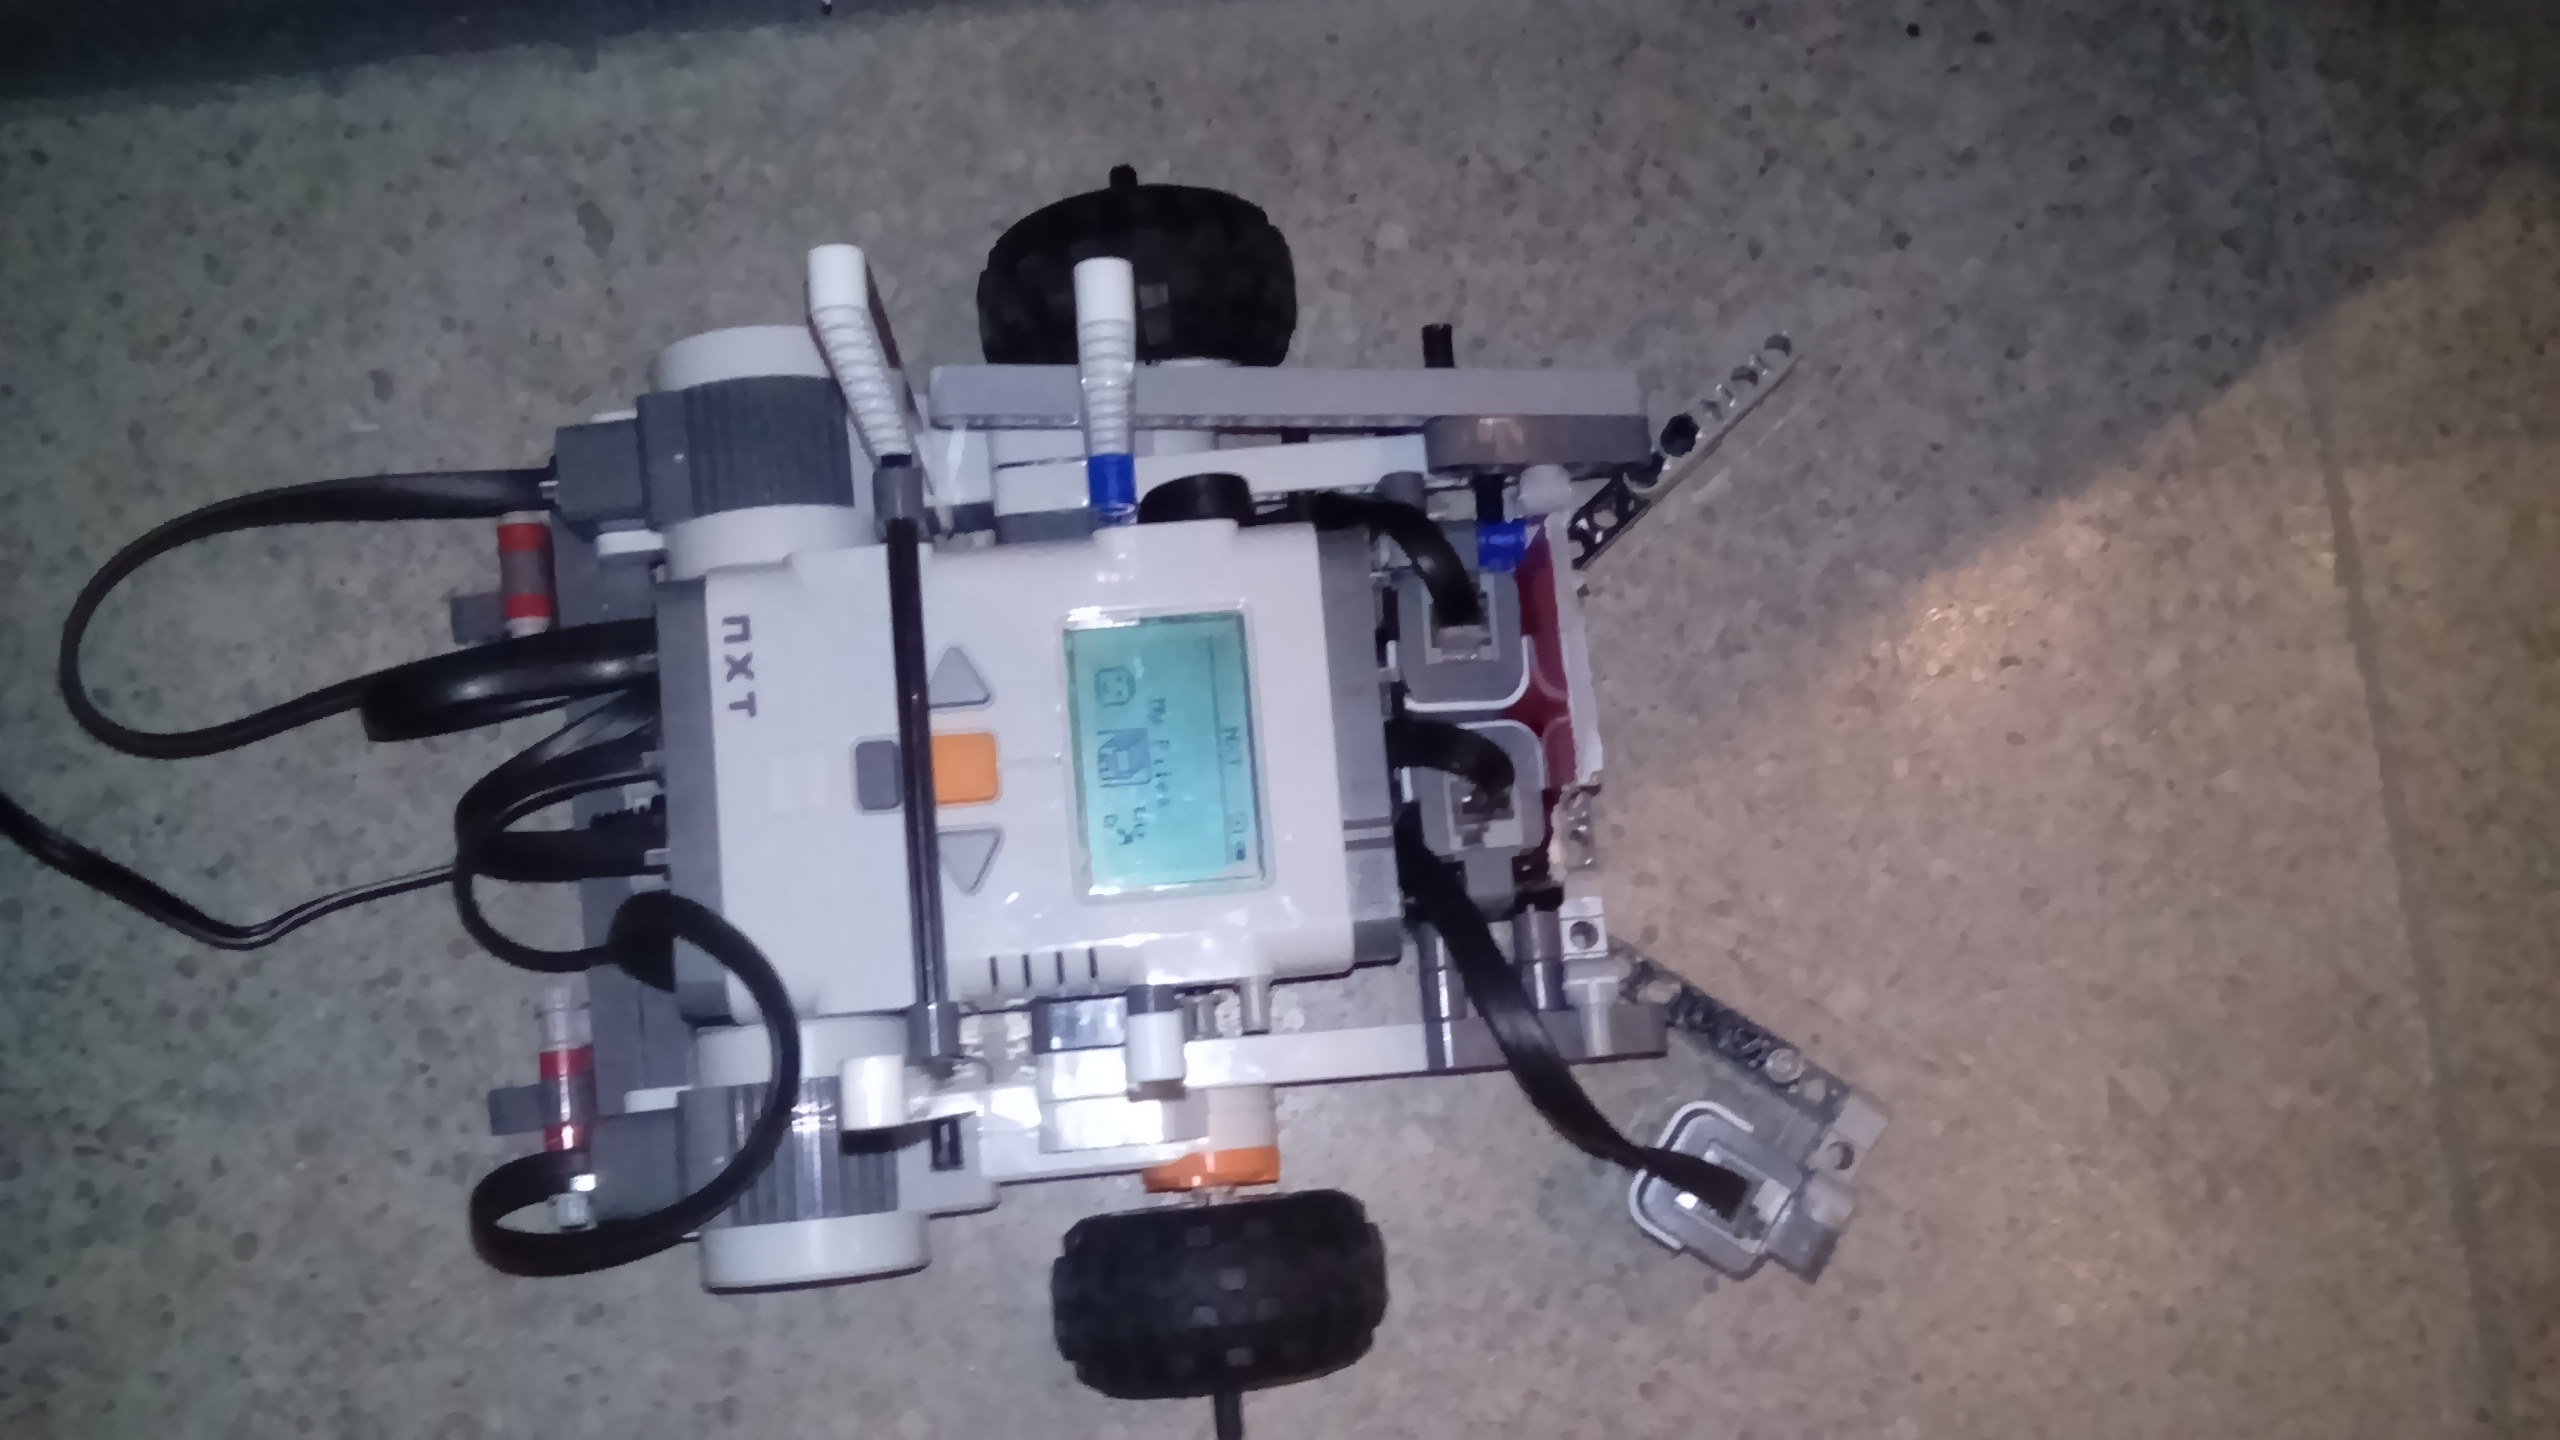
\includegraphics[scale = 0.1]{img/robot.jpg}
 \caption{Final design of the robot}
 \label{fig:final_robot}
\end{figure}


\subsection{Sensing}
In order to sense the world around it, the robot was fitted with three light sensors, the maximum number there was. Because there were only three light sensors, a decision had to be made on what to use the sensors for. All of the other types of sensors were deemed useless for this project.

It was quickly established that two sensors were needed for a line follow controller. The last sensor could then be used for a few things, e.g as indicator that a turn was completed or a detector of intersection. Both uses were tried and pros and cons were noted, and a decision was made on what was the best configuration. 

\subsection{Line Following}
To follow a line a proportional controller is used.
The light sensors gives a value to the controller and the speed of the motors are modified to be proportional to the error term between the two sensors.
The error term is calculated in equation \ref{eq:left_error}.

\begin{equation}
  \epsilon = \text{S}_{\text{left}} - \text{S}_{\text{right}}
 \label{eq:left_error}
\end{equation}
\begin{equation}
  V_\text{left} = V_\text{base} + P \epsilon
 \label{eq:left_speed}
\end{equation}
\begin{equation}
  V_\text{right} = V_\text{base} - P \epsilon
 \label{eq:right_speed}
\end{equation}

That error term is then multiplied by a constant, $P$, and added to the base speed, $V_\text{base}$.
The right motor gets the error term subtracted.
This allows for the motor to move at the base speed if the error term is zero and move towards the center of the line if it is not.
The robot configuration which generates this error can be seen in figure \ref{fig:line_follow}.

\nikolaj{Should this figure even exist? Maybe if it had arrows?}
\begin{figure}
 \begin{subfigure}{0.32\textwidth}
 \centering
    \begin{tikzpicture}
      \draw[ultra thick] (0,-1.5) to (0,1.5);
      \draw[ultra thick] (-1.5,0) to (1.5,0);
      
      \begin{scope}[rotate=-95]
	\draw node[robot,rotate=-95] at (0,0) {};
      \end{scope}
    \end{tikzpicture}
  \caption{Negative error term.}
 \end{subfigure}
 %
 \begin{subfigure}{0.32\textwidth}
 \centering
    \begin{tikzpicture}
      \draw[ultra thick] (0,-1.5) to (0,1.5);
      \draw[ultra thick] (-0.5,0) to (3.5,0);
      \draw[ultra thick] (3,-1.5) to (3,1.5);
      \node[name=P_r] at (0.5,0) {};
      \begin{scope}[rotate=-85]
	\draw node[robot,rotate=-85] at (P_r) {};
      \end{scope}
    \end{tikzpicture}
  \caption{Positive error term.}
 \end{subfigure}
 %
 \begin{subfigure}{0.32\textwidth}
 \centering
    \begin{tikzpicture}
      \draw[ultra thick] (0,-1.5) to (0,1.5);
      \draw[ultra thick] (-0.5,0) to (3.5,0);
      \draw[ultra thick] (3,-1.5) to (3,1.5);
      \node[name=P_r] at (1,0) {};
      
      \begin{scope}[rotate=-90]
	\draw node[robot,rotate=-90] at (P_r) {};
      \end{scope}
    \end{tikzpicture}
  \caption{Equilibrium.}
 \end{subfigure}
\caption{Error term as a result of the robot configuration.}
\label{fig:line_follow}
\end{figure}


\subsection{Turning}
To turn the robot a set of sub goals must be met.
If both motors turn in opposite direction, the robot will turn around the axis between the wheel.
This means the robot must be positioned with the axis over the intersection.
Then the robot can turn until the sensors in the middle of the robot sees the line.
As an extra calibration, the robot will then complete the turn by turning until the line is not visible anymore.
In figure \ref{fig:left_turn} is a left turn shown.
The final state of the turn is not perfect as the positioning of the sensors position cannot be placed in a perfect desired location.
This is compensated by the line following that is guaranteed to follow a turn.

\begin{figure}
 \begin{subfigure}{0.24\textwidth}
    \begin{tikzpicture}
      \draw[ultra thick] (0,-1.5) to (0,1.5);
      \draw[ultra thick] (-1.5,0) to (1.5,0);
      
      \begin{scope}[rotate=-90]
	\draw node[robot,rotate=-90] at (0,-1.25) {};
      \end{scope}
    \end{tikzpicture}
  \caption{Robot at line.}\label{left_turn_a}
  \end{subfigure}
%
 \begin{subfigure}{0.24\textwidth}
    \begin{tikzpicture}
      \draw[ultra thick] (0,-1.5) to (0,1.5);
      \draw[ultra thick] (-1.5,0) to (1.5,0);
      
      \begin{scope}[rotate=-90]
	\draw node[robot,rotate=-90] at (0,0) {};
      \end{scope}
    \end{tikzpicture}
  \caption{Center at axis.}\label{left_turn_b}
 \end{subfigure}
%
 \begin{subfigure}{0.24\textwidth}
    \begin{tikzpicture}
      \draw[ultra thick] (0,-1.5) to (0,1.5);
      \draw[ultra thick] (-1.5,0) to (1.5,0);
      
      \draw[red, very thick] (1,0) arc(0:65:1cm);
      \begin{scope}[rotate=-25]
	\draw node[robot,rotate=-25] at (0,0) {};
      \end{scope}
    \end{tikzpicture}
  \caption{Turn until line is found.}\label{left_turn_c}
 \end{subfigure}
%
 \begin{subfigure}{0.24\textwidth}
    \begin{tikzpicture}
      \draw[ultra thick] (0,-1.5) to (0,1.5);
      \draw[ultra thick] (-1.5,0) to (1.5,0);
      
      \begin{scope}[rotate=-5]
	\draw node[robot,rotate=-5,name=wallE] at (0,0) {};
      \end{scope}
      
      \draw[red, very thick] (wallE.north) arc(85:65:1cm);
    \end{tikzpicture}
  \caption{Turn until line is lost.}\label{left_turn_d}
 \end{subfigure}
 \caption{A left turn for the robot.}
 \label{fig:left_turn}
\end{figure}
